\documentclass[10pt,a4paper]{article}
\usepackage[latin1]{inputenc}
\usepackage{amsmath}
\usepackage{amsfonts}
\usepackage{amssymb}
\usepackage{graphicx}
\usepackage[caption=false,font=footnotesize]{subfig}
\usepackage{grffile}

\newcommand*\colvec[3][]{
	\begin{pmatrix}\ifx\relax#1\relax\else#1\\\fi#2\\#3\end{pmatrix}
}
\DeclareMathAlphabet{\mathpzc}{OT1}{pzc}{m}{it}

%\addtolength{\oddsidemargin}{-.875in}
%\addtolength{\evensidemargin}{-.875in}
%\addtolength{\textwidth}{1.75in}

%\addtolength{\topmargin}{-.875in}
%\addtolength{\textheight}{1.75in}

\title{STK9060 - Time Series \\ Dang Ha The Hien \\ Student number: 573543}

\begin{document}
	\maketitle
	\section{Problem 1}
To build an ARIMA model for the given data, I first inspect the time plot of the data, which given on top of Figure \ref{fig:mkts}. Obviously, the data is not stationary. There is an obvious trend, and the variance seems to increase over time. This suggests that we should use log transformation to first stabilize the variance. The time series after taking log is shown in the middle of Figure \ref{fig:mkts}. We see that the variance is now more stable, but the trend is still there. Therefore, I try to differentiate the log of mkts to detrend the series. The result is shown in the bottom of Figure \ref{fig:mkts}. I now refer to the differentiated log of mkts time series as mkgr, which is the quarterly growth rate of mkts. The time plot of mkgr shows that the time series is now relatively stable without any obvious trend. However, we can see that there seems to be different periods where the variances are significantly different. The time series variance is very large during 1980 to around $1992$. From 1993 to around 2007, the time series variance becomes very small. After 2008, the variance seems to increase again. This suggests that there could be a hidden state switching between those periods. I ignore those facts for now, and try to build an ARIMA model for the mkgr time series.

We now look at the sample ACF and PACF to identify appropriate autoregressive order $p$ and the moving average order $q$ for the ARIMA model. The plot is given in Figure \ref{fig:acf}. We see that the PACF is cutting off at lag 3, and the ACF is tailing off without any strong seasonal pattern. This suggests an AR(3) model. I also try an ARIMA(3,0,1) to see if an extra moving average term can help in this case. After fitting the two models, I get the result that ARIMA(3, 0, 0) has a smaller BIC score. However, the AIC and AICc both prefer the ARIMA(3, 0, 1) model. In this case, I choose the model ARIMA(3, 0, 0) to work on, since a simple model is probably more easily to be interpreted.

The estimated ARIMA(3, 0, 0) model is:
\begin{equation}
x_t = .0154_{(.0091)} + -.6277_{(.0766)} x_{t-1} -.4534_{(.0840)}- .3261_{(.0760)} + \hat{w}_t
\end{equation}
where $\hat{\sigma}_w = 0.0714$
\begin{figure}
	\centering
	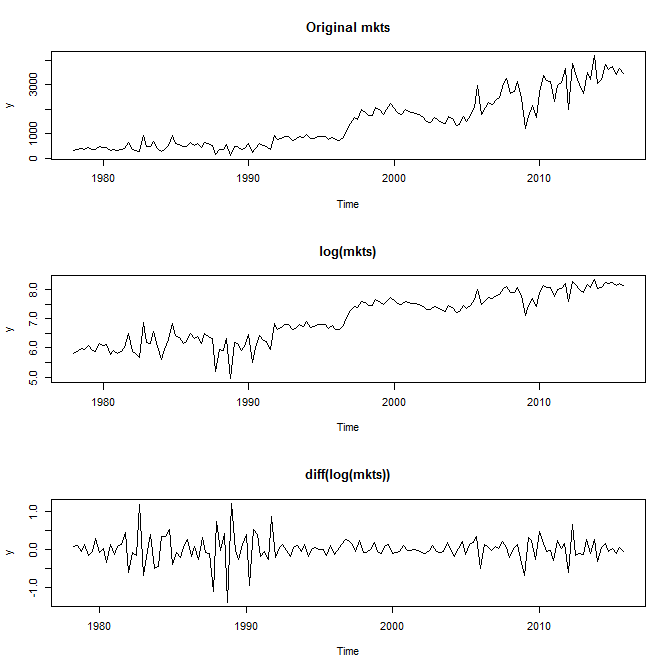
\includegraphics[width=10cm]{Figures/Problem1_mkts}
	\caption{\emph{Top:} time plot of the original mkts data. \emph{Middle:} mkts after taking log. \emph{Bottom:} mkts after differencing log}
	\label{fig:mkts}
\end{figure}
\begin{figure}
	\centering
	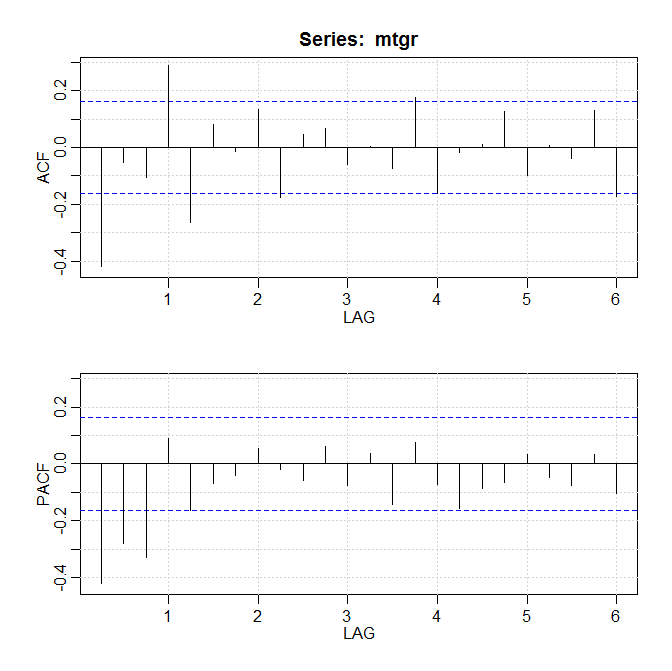
\includegraphics[width=10cm]{Figures/Problem1_acf}
	\caption{The sample ACF and PACF of the mkgr series. Lag is in terms of years.}
	\label{fig:acf}
\end{figure}
\subsection{Diagnostics for the fitted ARIMA(3, 0, 0) }
The plot of the ARIMA(3, 0, 0) residuals, its sample autocorrelation function, Q-Q plot, and Q-statistic are given in Figure \ref{fig:residual}. From the time plot of the standardized residuals, we see that there are 3 periods that have significant difference in variance, as indicated previously. Other than that, there is no obvious patterns. The residuals' ACF plot confirms this argument, as there is not significant correlation in the residuals time series. The Q-statistic tells the same story, which is never significant in the plot. The Q-Q plot shows that the residuals departure from normality at the tails due to outliers during the high variance periods. In general, the model fit the data pretty well, with the only problem is the difference in variance during different periods, which leads to fat tails of residuals distribution.

\begin{figure}
	\centering
	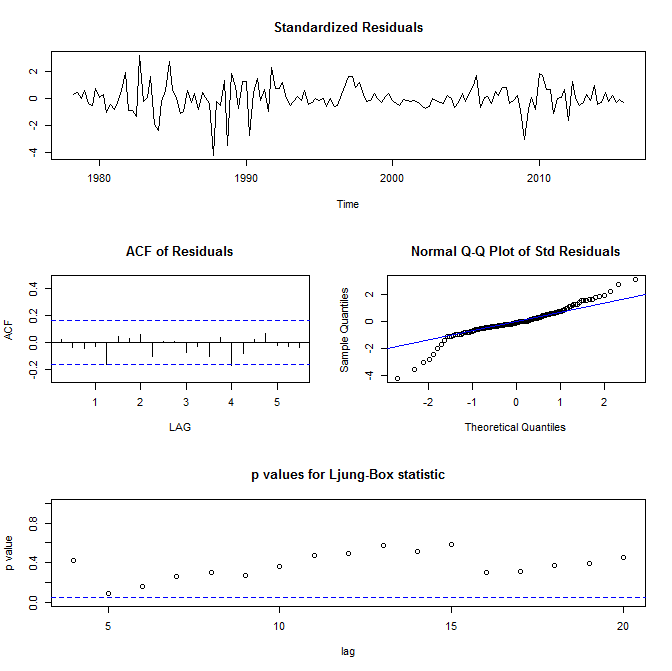
\includegraphics[width=10cm]{Figures/Problem1_residual}
	\caption{Diagnostics of the residuals from ARMA(3,0,0) fit on mkgr}
	\label{fig:residual}
\end{figure}

\subsection{Forecasting}
The forecast for the next two year of the mkts series using the above model is given in Figure \ref{fig:forecast}. Note that the figure is given in log scale.
\begin{figure}
	\centering
	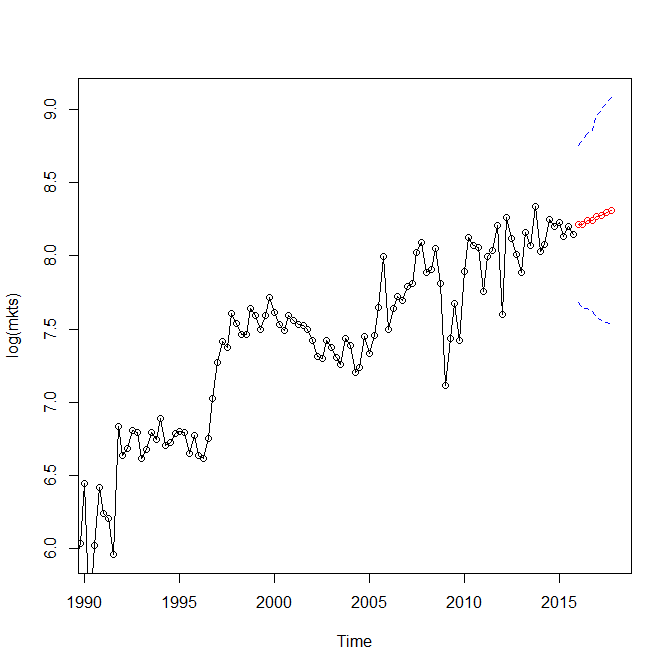
\includegraphics[width=10cm]{Figures/Problem1_forecast}
	\caption{Forecast for the next two year of log of the mkts series}
	\label{fig:forecast}
\end{figure}
	\section{Problem 2}
Given the weakly stationary ARMA(2,1) time series defined by:
\begin{equation}
x_t - 0.75x_{t-1} + 0.125x_{t-2} = w_t -0.2w_{t-1} \qquad w_t \sim N(0, \sigma_w^2)
\end{equation}
\subsection{Prove the model is causal and invertible}
The AR polynomial of the model is:
\begin{equation}
\Phi(z) = 1-0.75z+0.125z^2
\end{equation}
Which has two roots $z_1 = 2$ and $z_2 = 4$ which are all outside the unit circle. Therefore the model is \emph{causal}.

The MA polynomial of the model is:
\begin{equation}
\Theta(z) = 1 - 0.2z
\end{equation}
Which has one root $z = 5 > 1$. Therefore the model is invertible.

\subsection{Find the $\psi$-weights}
Since $x_t$ is causal, it can we represented by $x_t = \sum_{j=0}^{\infty} \psi_jw_{t-j}$. 

Let the polynomial of $\psi$-weights be $\Psi(z)$. Then the ARMA(2,1) and its linear process representation must match. In other words, the $\Phi(z)$, $\Theta(z)$ and $\Psi(z)$ must satisfy:
\begin{equation}
 \Phi(z)\Psi(z) = \Theta(z)
\end{equation}
Which can be expanded into:
\begin{equation}
(1-0.75z+0.125z^2)(\psi_0 + \psi_1z+\psi_2z^2...) = 1-0.2z
\end{equation}
By matching the coefficients, we can find the difference equation with initial conditions for $\psi$ as follow:
\begin{align*}
\psi_0 &= 1  && \text{matching constant}\\
\psi_1 - 0.75 \psi_0 &= -0.2 && \text{matching z}\\
\psi_j - 0.75 \psi_{j-1}+0.125\psi_{j-2} &= 0 &&\text{matching }z^j, (j \geq 2)
\end{align*}
From the first two equations, we get the initial conditions $\psi_0 = 1$ and $\psi_1 = 0.55$. The difference equation $\psi$-weights given in the last equation can be solved by finding the roots of its characteristic polynomial, which is 
\begin{equation}
1-0.75z+0.125z^2 = 0
\end{equation}

The above quadratic equation has two real distinct roots $z_1 = 2$ and $z_2 = 4$. Therefore, the general solution for $\psi$ is:
\begin{equation}
\psi_j = c_12^{-j} + c_2 4^{-j}
\end{equation}
We can find $c_1$ and $c_2$ by solving for the initial conditions:
\begin{equation}
\begin{split}
\psi_0 &= 1 = c_1 + c_2 \\
\psi_1 &= 0.55 = \frac{c_1}{2} + \frac{c_2}{4}
\end{split}
\end{equation}
Solving that, we get $c_1 = 1.2$ and $c_2 = -0.2$. Therefore, the $\psi$-weights are fully described by:
\begin{equation}\label{eq:psi_weight}
\psi_j = 1.2 \cdot 2^{-j} - 0.2 \cdot 4^{-j}
\end{equation}

\subsection{Find the $\gamma(h)$}
From the ARMA(2,1) equation:
\begin{equation}
x_t - 0.75x_{t-1} + 0.125x_{t-2} = w_t -0.2w_{t-1}
\end{equation}
By multiplying both sides by $x_{t-h}$ with $h\geq 0$ and take expectation, we get:
\begin{equation}
E(x_tx_{t-h}) -0.75E(x_{t-1}x_{t-h})+0.125E(x_{t-2}x_{t-h}) = E(w_t x_{t-h}) - 0.2E(w_{t-1}x_{t-h})
\end{equation}
Using the fact that the ARMA(2,1) is causal, or $E(w_tx_s) = 0$ when $t > s$, we can get the difference equation for $\gamma(h)$ and its initial conditions by evaluating the above equation at $h = 0$, $h=1$, $h=2$ and $h \geq 2$ respectively:
\begin{equation}
\begin{split}
(h = 0) \qquad &\gamma(0) - 0.75\gamma(1) + 0.125\gamma(2) = \sigma_w^2 - 0.2(0.75-0.2)\sigma_w^2 = 0.89\sigma_w^2  \\
(h=1) \qquad &\gamma(1) - 0.75\gamma(0) + 0.125\gamma(1) = -0.2\sigma^2_w\\
(h=2) \qquad &\gamma(2) - 0.75\gamma(1) + 0.125\gamma(0) = 0 \\ 
(h\geq 2) \qquad & \gamma(h) - 0.75\gamma(h-1) +0.125\gamma(h-2)=0 
\end{split}
\end{equation}
(Note that we use the property $\gamma(h) = \gamma(-h)$)

Solving the first three equations, we get the initial conditions: $\gamma(0) = 1.414\sigma_w^2$, $\gamma(1) = 0.765\sigma_w^2$ and $\gamma(2) = 0.397\sigma_w^2$. The fourth equation is the difference equation for $\gamma(h)$, which has the following characteristic polynomial:
\begin{equation}
1-0.75z+0.125z^2 = 0
\end{equation}
This quadratic equation has two real distinct roots $z_1 = 2$ and $z_2 = 4$. Therefore, the general solution for $\gamma(h)$ is $\gamma(h) = c_12^{-h} + c_24^{-h}$ for $h\geq 1$. To find $c_1$ and $c_2$, the general solution must satisfy the initial conditions, which leads to:
\begin{equation}
\begin{split}
\gamma(1) &= 0.765 \sigma_w^2 = \frac{c_1}{2} + \frac{c_2}{4}\\
\gamma(2) &= 0.397 \sigma_w^2 = \frac{c_1}{4} + \frac{c_2}{16} 
\end{split}
\end{equation}
Solving that we get $c_1 = 1.646 \sigma_w^2$ and $c_2 = -0.232\sigma_w^2$. Replace that to the general solution of $\gamma(h)$ we get:

\begin{equation} \label{eq:gamma_h}
\gamma(h) = \sigma_w^2(1.646 \cdot 2^{-h} - 0.232 \cdot 4^{-h})
\end{equation}

\subsection{Find $\gamma(h)$ of a general linear process}
Given a time series:
\begin{equation}
x_t = \sum_{j = -\infty}^{\infty} \psi_j w_{t-j}
\end{equation}
By definition, its autocovariance function $\gamma(h)$ is:
\begin{equation} \label{eq:gamma_linearprocess}
\begin{split}
\gamma(h) &= E(x_t x_{t+h}) \\
&= E(\sum_{j = -\infty}^{\infty} \psi_j w_{t-j} \sum_{k = -\infty}^{\infty} \psi_k w_{t-k+h})\\
&= E(\sum_{j = -\infty}^{\infty} \sum_{k = -\infty}^{\infty} \psi_j w_{t-j} \psi_k w_{t-k+h})\\
&= \sum_{j = -\infty}^{\infty} \sum_{k = -\infty}^{\infty}  \psi_j \psi_k E(w_{t-j} w_{t-k+h})
\end{split}
\end{equation}
Since $w_t$ is independent and identical distributed $N(0, \sigma_w^2)$, we have:
\begin{equation}
\begin{cases}
E(w_{t-j}w_{t-k+h}) = 0 &(k \neq j+h ) \\
E(w_{t-j}w_{t-k+h}) = \sigma_w^2 &( k = j+h)
\end{cases}
\end{equation}
Apply that to (\ref{eq:gamma_linearprocess}) we get:
\begin{equation}
\gamma(h) = \sigma_w^2  \sum_{j = -\infty}^{\infty} \psi_j \psi_{j+h}
\end{equation}
Which is what we are looking for.

\subsection{Find $\gamma(h)$ from linear process representation}
The linear process representation of ARMA(2, 1) was derived in (\ref{eq:psi_weight}) as:
\begin{equation}
\psi_j = 1.2 \cdot 2^{-j} - 0.2 \cdot 4^{-j}
\end{equation}
From this representation, we can easily derive the $\gamma(h)$ function using the formula derived in the previous question:

\begin{equation}
\begin{split}
\gamma(h) &= \sigma_w^2  \sum_{j = -\infty}^{\infty} \psi_j \psi_{j+h} \\
&= \sigma_w^2  \sum_{j = 0}^{\infty} (1.2 \cdot 2^{-j} - 0.2 \cdot 4^{-j})(1.2 \cdot 2^{-(j+h)} - 0.2 \cdot 4^{-(j+h)})\\
&= \sigma_w^2  \sum_{j = 0}^{\infty}(1.2^2 \cdot 2^{-2j} - 1.2\cdot 0.2 \cdot 2^{-3j})2^{-h} + (0.2^2 \cdot 2^{-4j} - 1.2 \cdot 0.2 \cdot 2^{-3j})4^{-h}
\end{split}
\end{equation}

We have that $\sum_{j=0}^{\infty} a^j = \frac{1}{1-a}$ if $a < 1$. Apply that to the above equation, we get:

\begin{equation}
\begin{split}
\gamma(h) &= \sigma_w^2 [(\frac{1.2^2}{1-2^{-2}} - \frac{1.2\cdot 0.2}{1-2^{-3}})2^{-h} + (\frac{0.2^2}{1-2^{-4}}-\frac{1.2\cdot 0.2}{1-2^{-3}})4^{-h}]\\
 &= \sigma_w^2(1.646 \cdot 2^{-h} - 0.232 \cdot 4^{-h})
\end{split}
\end{equation}

Which is identical to what we got in (\ref{eq:gamma_h}).
	\section{Problem 3}
Let $x_1, ..., x_n$ be observations from a stationary time series $\{x_t\}$ with covariance function $\gamma_x(h)$. Its spectral density, discreet Fourier transform, and the periodogram are defined respectively as:

\begin{equation}
\begin{split}
f_x(\omega) &= \sum_{h=-\infty}^{\infty} \gamma_x(h) e^{-2\pi i \omega h}\\
d_f(\omega_j) &= \frac{1}{\sqrt{n}}\sum_{t = 1}^{n} x_t e^{-2\pi i \omega_j t}\\
I_f(\omega_j) &= |d_f(\omega_j)|^2
\end{split}
\end{equation}
With $\omega_j = j/n, j = 0, ..., n-1$ are Fourier coefficients.

\subsection{Prove that periodogram $I_f(\omega_j)$ is a sample version of spectral density $f_x(\omega)$}
First we rewrite the DFT of $x_t$ to:
\begin{equation}
d_f(\omega_j) = \frac{1}{\sqrt{n}} \sum_{t=1}^{n} (x_t - \bar{x}) e^{-2\pi i \omega_j t} \qquad (j > 0)
\end{equation}
With $\bar{x}$ is the mean of $x$. The result is derived by the fact that $\bar{x}\sum_{t = 1}^{n} e^{-2\pi i \frac{j}{n} t} = 0$ when $j > 0$ \footnote{We can prove this easily by using the sum of geometric series}.

By definition, for $j > 0$, the periodogram can be found by:
\begin{equation}
\begin{split}
I_f(\omega_j) &= |d_f(\omega_j)|^2 \\
&= \frac{1}{n} \sum_{t = 1}^{n} (x_t- \bar{x}) e^{-2\pi i \omega_j t} \sum_{s = 1}^{n} ((x_s - \bar{x})e^{-2\pi i \omega_j s})^* \\
&= \frac{1}{n} \sum_{t=1}^{n} \sum_{s=1}^{n} (x_t- \bar{x}) (x_s - \bar{x})e^{-2\pi i \omega_j (t-s)}
\end{split}
\end{equation}
Note that conjugate of sum is sum of conjugate. Now by defining $h = t-s$, we can get:
\begin{equation}
\begin{split}
I_f(\omega_j) &= \frac{1}{n} \sum_{t=1}^{n} \sum_{h=t-1}^{t-n} (x_t - \bar{x})(x_{t-h} - \bar{x})e^{-2\pi i \omega_j h}\\
&= \frac{1}{n} \sum_{h=-(n-1)}^{0}\sum_{t=1}^{n+h}(x_t - \bar{x})(x_{t-h} - \bar{x})e^{-2\pi i \omega_j h} \\
&+ \frac{1}{n}\sum_{h=1}^{n-1}\sum_{t=h+1}^{n}(x_t - \bar{x})(x_{t-h} - \bar{x})e^{-2\pi i \omega_j h}
\end{split}
\end{equation}
In the last equation, we split $h$ into two cases $h \leq 0$ and $h > 0$, which allows us to change the summing order. Now for the first term, we apply the fact that $h \leq 0$, and for the second term, we change the index to $t' = t - h$, which leads to.

\begin{equation}
\begin{split}
I_f(\omega_j) &= \frac{1}{n} \sum_{h=-(n-1)}^{0}\sum_{t=1}^{n-|h|}(x_t - \bar{x})(x_{t+|h|} - \bar{x})e^{-2\pi i \omega_j h} \\
&+ \frac{1}{n}\sum_{h=1}^{n-1}\sum_{t'=1}^{n-h}(x_{t'+h} - \bar{x})(x_{t'} - \bar{x})e^{-2\pi i \omega_j h}
\end{split}
\end{equation}
Now we can merge two terms together, using the fact that for the second term $h > 0$.
\begin{equation} \label{eq:periodogram_sample}
I_f(\omega_j) = \frac{1}{n} \sum_{h=-(n-1)}^{n-1}\sum_{t=1}^{n-|h|}(x_t - \bar{x})(x_{t+|h|} - \bar{x})e^{-2\pi i \omega_j h}
\end{equation}

By definition, the estimate of the covariance is given by:
\begin{equation}
\hat{\gamma}_x(h) = \frac{1}{n}\sum_{t=1}^{n-|h|}(x_t - \bar{x})(x_{t+|h|} - \bar{x})
\end{equation}

Therefore, the periodogram is equal to:
\begin{equation}
\begin{split}
I_f(\omega_j) &= \sum_{h=-(n-1)}^{n-1}\hat{\gamma}_x(h) e^{-2\pi i \omega_j h} \\
&= \sum_{|h|<n}\hat{\gamma}_x(h) e^{-2\pi i \omega_j h} \qquad (j > 0)
\end{split}
\end{equation}
Which shows that periodogram is the sample version of the spectral density. This is also what we are looking for.

When $j = 0$, $d_f(0) = \frac{1}{\sqrt{n}}\sum_{t = 1}^{n} x_t$. Therefore:

\begin{equation}
I_f(0) = (\frac{1}{\sqrt{n}}\sum_{t = 1}^{n} x_t)^2 = n\bar{x}^2
\end{equation}

\subsection{Find expectation of periodogram}
Let $\mu$ be the population mean of $x_t$. Without changing anything, we can replace $\bar{x}$ by $\mu$ in the equation (\ref{eq:periodogram_sample})\footnote{In fact, we can replace $\bar{x}$ by any constant}. By taking the expectation on both sides, the equation (\ref{eq:periodogram_sample}) becomes:

\begin{equation}\label{eq:expectation_periodogram}
\begin{split}
E[I_f(\omega_j)] &= \frac{1}{n} \sum_{h=-(n-1)}^{n-1}\sum_{t=1}^{n-|h|}E((x_t - \mu)(x_{t+|h|} - \mu))e^{-2\pi i \omega_j h} \\
&= \frac{1}{n} \sum_{h=-(n-1)}^{n-1}\sum_{t=1}^{n-|h|} \gamma_x(h) e^{-2\pi i \omega_j h}\\
&= \sum_{|h|<n}(1-\frac{|h|}{n})\gamma_x(h) e^{-2\pi i \omega_j h} \qquad (j > 0)
\end{split}
\end{equation}
Which is what we are looking for.

When $j = 0$, we have 
\begin{equation} \label{eq:I_0_expectation}
E[I_f(0)] = E[d_f(0)^2] = E[(\frac{1}{\sqrt{n}}\sum_{t = 1}^{n} x_t)^2] =n(\mu^2+ var(\bar{x}))
\end{equation}

\subsection{Show a smooth version of periodogram is reasonable}
First, we try to derive the variance of $I_f(\omega_j)$ when $n \rightarrow \infty$. Using the Appendix C.2 in the book, and the central limit theorem, we know that the distribution of cosine and sine transform of $x_t$ converge to independent normal distributions with zero mean and variances approximately equal to one half of the theoretical spectrum:

\begin{equation}
\begin{split}
d_c(\omega_j) &\xrightarrow{d} AN(0, f_x(\omega)/2) \\
d_s(\omega_j) &\xrightarrow{d} AN(0, f_x(\omega)/2) \\
\end{split}
\end{equation}
Since $I_f(\omega_j) = d_c(\omega_j)^2 + d_s(\omega_j)^2$, which is sum of squares of two independent normal random variables. Therefore, the asymptotic distribution of the periodogram is given by:
\begin{equation}
I_f(\omega_j) \xrightarrow{d} \frac{f_x(\omega)}{2} \chi^2_2
\end{equation}
Therefore, the asymptotic variance of the periodogram is:
\begin{equation}
var(I_f(\omega_j)) \rightarrow 2 f^2_x(\omega)
\end{equation} 

Now, instead of directly using raw periodogram $I_f(\omega_j)$ to estimate the spectral density, we use the suggested estimator:
\begin{equation}
\hat{g}(\omega_j) = \sum_{|h|<n}(1-\frac{|h|}{n})\hat{\gamma}_x(h)e^{-2\pi i \omega_j h}
\end{equation}

We see that the above estimator follows the following lag window form:
\begin{equation}
\tilde{f}(\omega) = \sum_{|h|\leq r}w(\frac{h}{r})\hat{\gamma}_x(h)e^{-2\pi i \omega h}
\end{equation}

In this case, $r = n$, and the weight function $w(\frac{h}{n}) = w(x) = 1-|x|$.

This weight function satisfies that $w(0) = 1; |w(x)| \leq 1$ and $w(x) = w(-x)$. Therefore, we can apply the asymptotic theory for estimators in the lag window form (with $r = n$)

\begin{equation}
\begin{split}
 var(\hat{g}(\omega_j) ) &\rightarrow \frac{n}{n} f_x^2(\omega) \int_{-1}^{1}w^2(x) dx \qquad \omega \neq 0, 1/2 \\
&\rightarrow  f_x^2(\omega) \int_{-1}^{1}(1-|x|)^2 dx \\
&\rightarrow \frac{2}{3} f_x^2(\omega) 
\end{split}
\end{equation}
We see that the estimator $\hat{g}(\omega_j)$ has smaller asymptotic variance: $\frac{2}{3} f_x^2(\omega)$, comparing to the raw periodogram estimator $I_f(\omega_j)$, which has asymptotic variance of 2 $f^2_x(\omega_j)$. This makes $\hat{g}(\omega_j)$ a more reasonable estimator, comparing to the raw periodogram.

\subsection{Show that expectation of periodogram converge to spectral density}
From the expectation of periodogram derived in (\ref{eq:expectation_periodogram}), we have:
\begin{equation} \label{eq:expectation_periodogram_converge}
\begin{split}
E[I_f(\omega_j)] &= \sum_{|h|<n}(1-\frac{|h|}{n})\gamma_x(h) e^{-2\pi i \omega_j h} \\
&= \sum_{|h|<n}\gamma_x(h)e^{-2\pi i \omega_j h}  - \frac{\sum_{|h|<n} |h|\gamma_x(h)e^{-2\pi i \omega_j h}}{n}  \qquad (j > 0)
\end{split}
\end{equation}

When $n \rightarrow \infty$, we now try to prove that if we assume:
\begin{equation} \label{eq:periodogram_regularity_cond}
\sum_{h = - \infty}^{\infty} |h||\gamma_x(h)| = \theta < \infty
\end{equation}
then the sum $\sum_{h = -\infty}^{h = \infty} |h|\gamma_x(h)e^{-2\pi i \omega_j h}$ is also bounded, which makes the second term in (\ref{eq:expectation_periodogram_converge}) vanishes when $n \rightarrow \infty$.

We have
\begin{equation}
|h|\gamma_x(h) \leq |h||\gamma_x(h)| \leq \sum_{h = - \infty}^{\infty} |h||\gamma_x(h)| = \theta \qquad \forall h
\end{equation}
Therefore, we have:
\begin{equation}
\sum_{h = -\infty}^{h = \infty} |h|\gamma_x(h)e^{-2\pi i \omega_j h} \leq \theta \sum_{h = -\infty}^{h = \infty}e^{-2\pi i \omega_j h}
\end{equation}

Since $-1/2<\omega_j<1/2$ and $\omega_j \neq 0$, we have: $|e^{2\pi i \omega_j}| < 1$ and $|e^{-2\pi i \omega_j}| < 1$, which enough for us to bound the sum:
\begin{equation}
\begin{split}
\sum_{h = -\infty}^{h = \infty}e^{-2\pi i \omega_j h} &= \sum_{h = 0}^{h = \infty}e^{-2\pi i \omega_j h} + \sum_{h = 1}^{h = \infty}e^{2\pi i \omega_j h} \\
&= \frac{1}{1-e^{-2\pi i \omega_j}} + \frac{1}{1-e^{2\pi i \omega_j}} - 1 < \infty
\end{split}
\end{equation}

Therefore, we have proved that under the condition (\ref{eq:periodogram_regularity_cond}), the sum $\sum_{h = -\infty}^{h = \infty} |h|\gamma_x(h)e^{-2\pi i \omega_j h}$ is bounded. Apply this result to (\ref{eq:expectation_periodogram_converge}) and let $n \rightarrow \infty$, we have:
\begin{equation}
\begin{split}
E[I_f(\omega_j)] &\rightarrow \sum_{h = -\infty}^{\infty} \gamma_x(h)e^{-2\pi i \omega_j h}  - 0 \\
&\rightarrow f_x(\omega) \qquad \qquad (\omega \neq 0)
\end{split}
\end{equation}
With the assumed regularity condition in (\ref{eq:periodogram_regularity_cond}), which is:
\begin{equation}
\sum_{h = - \infty}^{\infty} |h||\gamma_x(h)| = \theta < \infty
\end{equation}

For the case $\omega = 0$, as shown in (\ref{eq:I_0_expectation}), 
\begin{equation}
E[I_f(0)] - n\mu^2 = n\cdot var(\bar{x}) \rightarrow \sum_{h = -\infty}^{h = \infty}\gamma_x(h) = f_x(0)
\end{equation}

	\section{Problem 4}
The Holt-Winters forecasting and recursive updating scheme are given by:
\begin{equation}
\begin{split} \label{eq:HW}
x^{t-1}_t &= m_{t-1} + b_{t-1}\\
m_t &= \lambda_0x_t + (1-\lambda_0)(m_{t-1}+b_{t-1})\\
b_t &= \lambda_1(m_t - m_{t-1}) + (1-\lambda_1)b_{t-1}  \\
\end{split}
\end{equation}
\subsection{Why the updating formula of $b_t$ is reasonable?}
We see that $x_t$ is forecasted as sum of the current estimate of the local level $m_{t-1}$ and the local slope $b_{t-1}$. The new local level $m_t$ is updated (i.e. estimated) as the weighted average of the prediction $x^{t-1}_t$ and the actual value $x_t$. The new local linear trend $b_t$ is then updated as the weighted average of the new trend (i.e. growth) $m_t - m_{t-1}$ and the last estimated trend $b_{t-1}$. Therefore, the updating formula of $b_t$ in (\ref{eq:HW}) estimates the local trend by smoothing the observed trend exponentially, which is reasonable.

To get the initial values $b_2$ and $m_2$, assume that we have observed $x_1$ and $x_2$, and the innovations (i.e. prediction errors) $\epsilon_0 = \epsilon_1 = 0$, we then have:

\begin{equation}
\begin{split}
x_1 &= m_0 + b_0\\
x_2 &= m_1 + b_1\\
m_2 &= \lambda_0 x_2 + (1-\lambda_0) (m_1 + b_1) = x_2\\
m_1 &= \lambda_0 x_1 + (1-\lambda_0) (m_0 + b_0) = x_1\\
b_1 &= x_2 - m_1 = x_2 - x_1\\
b_2 &= \lambda_1 (m_2 - m_1) + (1-\lambda_1)b_1 = x_2 - x_1\\
\end{split}
\end{equation}

Therefore, reasonable starting values are $m_2 = x_2$ and $b_2 = x_2 - x_1$,  which makes sense since $m_2$ is the local level and $b_2$ is local linear trend at $t = 2$.

\subsection{Rearrange the updating formulas}
Having $x^{t-1}_t = m_{t-1} + b_{t-1}$, we can rearrange the updating formula for $m_t$ as following:
\begin{equation}
\begin{split}
m_t &= \lambda_0 x_t + (1-\lambda_0)(m_{t-1}+b_{t-1}) \\
\Leftrightarrow m_t &= \lambda_0 x_t + m_{t-1}+b_{t-1} - \lambda_0(m_{t-1}+b_{t-1}) \\ 
\Leftrightarrow m_t &= m_{t-1} +  b_{t-1} + \lambda_0(x_t - x^{t-1}_t) \\
\end{split}
\end{equation}

This leads to the following updating formula for $b_t$:
\begin{equation}
\begin{split}
b_t &= \lambda_1(m_t - m_{t-1}) + (1-\lambda_1)b_{t-1} \\
\Leftrightarrow b_t &= \lambda_1(b_{t-1} +\lambda_0(x_t - x^{t-1}_t)) + (1-\lambda_1)b_{t-1}\\
\Leftrightarrow b_t &= b_{t-1} + \lambda_0\lambda_1 (x_t - x^{t-1}_t)
\end{split}
\end{equation}

I now define the innovation series as $e_t = x_t - x^{t-1}_t$, which simplifies the updating formulas and is useful for later questions:
\begin{equation} \label{eq:update_HW}
\begin{split}
e_t &= x_t - x^{t-1}_t\\
m_t &= m_{t-1} +  b_{t-1} + \lambda_0e_t\\
b_t &= b_{t-1} + \lambda_0\lambda_1 e_t
\end{split}
\end{equation}
\subsection{Express the local linear trend model on state-space form}
The local linear trend model is given by:
\begin{equation} \label{eq:llt}
\begin{split}
y_t &= \mu_t + \epsilon_t \\
\mu_t &= \mu_{t-1} + \beta_{t-1} + \eta_t\\
\beta_t &= \beta_{t-1} + \zeta_t
\end{split}
\end{equation}
where $\epsilon_t, \eta_t, \zeta_t$ are independent with $\epsilon_t \sim N(0, 1), \eta_t \sim N(0, \sigma_\eta^2), \zeta_t \sim N(0, \sigma_\zeta^2)$.

We can express the local linear trend model in (\ref{eq:llt}) in the matrix form:
\begin{equation}
\begin{split}
y_t &= \begin{pmatrix}1 & 0\end{pmatrix}\colvec{\mu_t}{\beta_t} + \epsilon_t\\
\colvec{\mu_t}{\beta_t} &= \begin{pmatrix}1 & 1\\0 & 1\end{pmatrix} \colvec{\mu_{t-1}}{\beta_{t-1}} +  \colvec{\eta_t}{\zeta_t}
\end{split}
\end{equation}

Therefore, if we define $x_t = \colvec{\mu_t}{\beta_t}$ as the state vector, we can then express the model by the two following transition and measurement equations:
\begin{align*}
y_t &= \begin{pmatrix}1 & 0\end{pmatrix} x_t + \epsilon_t & \epsilon_t &\sim N(0, 1)\\
x_t &= \begin{pmatrix}1 & 1\\0 & 1\end{pmatrix} x_{t-1} +  \colvec{\eta_t}{\zeta_t} & \colvec{\eta_t}{\zeta_t} &\sim N(0, \begin{pmatrix}\sigma_\eta^2 & 0\\0 & \sigma_\zeta^2\end{pmatrix})
\end{align*}
Therefore, the above local linear trend model can be fully described in state-space form using the following parameters:
\begin{equation} \label{eq:statespace_para}
\begin{split}
\Phi &= \begin{pmatrix}1 & 1\\0 & 1\end{pmatrix}\\
A &=  \begin{pmatrix}1 & 0\end{pmatrix}\\
Q &= \begin{pmatrix}\sigma_\eta^2 & 0\\0 & \sigma_\zeta^2\end{pmatrix} \\
R &= 1
\end{split}
\end{equation}
\subsection{Kalman filter}
With the parameters given in (\ref{eq:statespace_para}), and assume that the starting values of the state is $x_0 \sim N(\colvec{\mu_0}{\beta_0}, P_0^0)$, the Kalman filter for $x_t$ is given as following.

Assume that we have observed data until $t-1$, first we make prediction for the next state: $x^{t-1}_t$, its variance matrix $P^{t-1}_t$, and prediction of the observable data $y^{t-1}_{t}$
\begin{equation}
\begin{split}
x^{t-1}_t &= \Phi x^{t-1}_{t-1}\\
P^{t-1}_t &= \Phi P^{t-1}_{t-1}\Phi'+Q\\
y^{t-1}_t &= Ax^{t-1}_t
\end{split}
\end{equation}
Then after observing $y_t$, we calculate the innovation $e_t$ (prediction errors), and use that to update the state vector, using the fact that the innovation has correlation with the state. The optimal updating scheme is given by the following Kalman filter:
\begin{equation} \label{eq:Kalman_filter}
\begin{split}
e_t &= y_t - y^{t-1}_t = y_t - Ax^{t-1}_t \\
\Sigma_t &= var(e_t) = AP^{t-1}_{t}A'+ R \\
K_t &= P^{t-1}_tA'\Sigma_t^{-1}\\
P^t_t &= [I - K_tA]P^{t-1}_t\\
x^t_t &= x^{t-1}_t + K_te_t\\
\end{split}
\end{equation}

We see that the new estimate of the state $x^t_t$ is the combination of its prediction $x^{t-1}_{t}$ and the prediction error $e_t$, under the Kalman gain $K_t$. This is quite similar to the updating scheme of Holt-Winters model that we obtained in (\ref{eq:update_HW}). I will exploit this fact in the later question.
\subsection{Kalman smoother}
After observing $y_t$ for $t = 1, ..., n$, we can estimate the state using all these observed data, which is call smoothing. To run the Kalman smoother, we must first run the Kalman filter forward (from $t=1$ to $t=n$), and then run the following Kalman smoother backward (from $t=n-1$ to $t=1$) with the initial value $x^n_n$ and $P^n_n$:

\begin{equation}
\begin{split}
x^n_{t-1} &= x^{t-1}_{t-1} + J_{t-1}(x^n_t - x^{t-1}_t) \\
P^n_{t-1} &= P^{t-1}_{t-1} + J_{t-1}(P^n_t-P^{t-1}_t)J'_{t-1}\\
J_{t-1} &= P^{t-1}_{t-1}\Phi'[P^{t-1}_t]^{-1}\\
\end{split}
\end{equation}

\subsection{Steady state of the Kalman filter}
I first assume that the regularity conditions are satisfied by our local linear trend model, so that its Kalman filter can reach the steady state after some finite number of time steps. At this steady state, the state error covariance matrix $P^{t-1}_{t}$ must converge to a time invariant matrix, or $P^{t-1}_{t} = P$ 

Following the Kalman filter given in (\ref{eq:Kalman_filter}), we have:
\begin{equation}
\begin{split}
	P^{t+1}_t &= \Phi P^{t-1}_{t-1} \Phi' + Q\\
\Leftrightarrow P^{t+1}_t &= \Phi [I - K_tA]P^{t-1}_t \Phi' + Q\\
\Leftrightarrow P^{t+1}_t &= \Phi [I - P^{t-1}_tA'\Sigma_t^{-1}A]P^{t-1}_t \Phi' + Q \\
\Leftrightarrow P^{t+1}_t &= \Phi [I - P^{t-1}_tA'(AP^{t-1}_{t}A'+ R)^{-1}A]P^{t-1}_t \Phi' + Q
\end{split}
\end{equation}
Using the fact that the $P^{t-1}_t$ matrix has already converged at the steady state, we have $P^{t+1}_t = P^{t-1}_t = P$. Replace that into the above formula, we have:
\begin{equation}\label{eq:Ricatti}
\begin{split}
&P^{t+1}_t = \Phi [I - P^{t-1}_tA'(AP^{t-1}_{t}A'+ R)^{-1}A]P^{t-1}_t \Phi' + Q\\
\Leftrightarrow &P = \Phi[I - PA'(APA'+R)^{-1}A]P \Phi'+Q \\
\Leftrightarrow & P - \Phi P \Phi' +\Phi PA'(APA'+R)^{-1}AP \Phi'-Q = 0
\end{split}
\end{equation}
Which is the Ricatti equation.

\subsection{Steady state Kalman filter vs. Holt-Winter updating scheme}
At the steady state, the Kalman gain also converges to $K_t = K$. Let $K = \colvec{K_1}{K_2}$, the Kalman filter can be written as:
\begin{equation}
\begin{split}
x^t_t &= x^{t-1}_t + Ke_t \\
\Leftrightarrow x^t_t &= \Phi x^{t-1}_{t-1} + Ke_t\\
\Leftrightarrow \colvec{\mu_t}{\beta_t} &= \begin{pmatrix}1 & 1\\0 & 1\end{pmatrix} \colvec{\mu_{t-1}}{\beta_{t-1}} + \colvec{K_1 e_t}{K_2 e_t}\\
\Leftrightarrow \colvec{\mu_t}{\beta_t}& = \colvec{\mu_{t-1}+\beta_{t-1}}{\beta_{t-1}} + \colvec{K_1}{K_2}e_t
\end{split}
\end{equation}

Now looking at the Holt-Winters updating scheme derived in (\ref{eq:update_HW}):
\begin{equation}
\begin{split}
m_t &= m_{t-1} +  b_{t-1} + \lambda_0e_t\\
b_t &= b_{t-1} + \lambda_0\lambda_1 e_t
\end{split}
\end{equation}

 We see that from the above Kalman filter at the steady state, if we replace $\mu_t$ by $m_t$ and $\beta_t$ by $b_t$, and set $K_1 = \lambda_0$ and $K_2 = \lambda_0\lambda_1$, we will get the exact Holt-Winters updating formulas.

\subsection{Find P given $\lambda_0$ and $\lambda_1$}
At the steady state, let $P_t = P = \begin{pmatrix}p_{11} & p_{12}\\p_{12} & p_{22}\end{pmatrix}$ (since $P$ is symmetric). At the steady state, $K_t$ and $\Sigma_t$ will also converge to $K_t = K$ and $\Sigma_t = \Sigma$. From the Kalman filter formulas, we have:

\begin{equation} \label{eq:Kconditions}
\begin{split}
\Sigma &= APA' + R = \begin{pmatrix}1 & 0\end{pmatrix} \begin{pmatrix}p_{11} & p_{12}\\p_{12} & p_{22}\end{pmatrix}  \colvec{1}{0} + 1 = p_{11} + 1 \\
K &= PA'\Sigma^{-1} = \frac{\begin{pmatrix}p_{11} & p_{12}\\p_{12} & p_{22}\end{pmatrix} \colvec{1}{0}}{p_{11}+1} = \frac{\colvec{p_{11}}{p_{12}}}{p_{11}+1}
\end{split}
\end{equation}
Therefore, we have $K_1 = \frac{p_{11}}{p_{11}+1}$ and $K_2 = \frac{p_{12}}{p_{11}+1}$

From the previous question, if we want our Kalman filter converges to the Holt-Winter updating scheme at its steady state, we must have $K_1 = \lambda_0$ and $K_2 = \lambda_0\lambda_1$. This leads to the following conditions on $p_{11}$and $p_{12}$:

\begin{equation}\label{eq:Pconditions}
\begin{split}
K_1 &= \frac{p_{11}}{p_{11}+1} = \lambda_0 \\
K_2 &= \frac{p_{12}}{p_{11}+1} = \lambda_0 \lambda_1 \\
\end{split}
\Leftrightarrow 
\begin{split}
p_{11} &= \frac{\lambda_0}{1-\lambda_0} \\
p_{12} &= \frac{\lambda_0\lambda_1}{1-\lambda_0}
\end{split}
\end{equation}

\subsection{Relationship between $\sigma_\eta^2$, $\sigma_\zeta^2$ and $\lambda_0$, $\lambda_1$}
The Ricatti equation derived in (\ref{eq:Ricatti}):
\begin{equation}
\begin{split}
&P - \Phi P \Phi' +\Phi PA'(APA'+R)^{-1}AP \Phi'-Q = 0 
\end{split}
\end{equation}
can be expanded by the following facts:
\begin{equation}
\begin{split}
\Phi P \Phi' &= \begin{pmatrix}1 & 1\\0 & 1\end{pmatrix} \begin{pmatrix}p_{11} & p_{12}\\p_{12} & p_{22}\end{pmatrix} \begin{pmatrix}1 & 0\\1 & 1\end{pmatrix} = \begin{pmatrix}p_{11} + 2p_{12}+p_{22}& p_{12}+p_{22}\\p_{12}+p_{22} & p_{22}\end{pmatrix} \\
\Phi PA' &= \begin{pmatrix}1 & 1\\0 & 1\end{pmatrix} \begin{pmatrix}p_{11} & p_{12}\\p_{12} & p_{22}\end{pmatrix} \colvec{1}{0} = \begin{pmatrix}p_{11} +p_{12}\\p_{12}\end{pmatrix} \\
APA' + R &= \begin{pmatrix}1 & 0\end{pmatrix} \begin{pmatrix}p_{11} & p_{12}\\p_{12} & p_{22}\end{pmatrix}  \colvec{1}{0} + 1 = p_{11} + 1 \\
AP\Phi' &= \begin{pmatrix}1 & 0\end{pmatrix} \begin{pmatrix}p_{11} & p_{12}\\p_{12} & p_{22}\end{pmatrix} \begin{pmatrix}1 & 0\\1 & 1\end{pmatrix} = \begin{pmatrix}p_{11} +p_{12} & p_{12}\end{pmatrix} 
\end{split}
\end{equation}

The Ricatti equation becomes:
\begin{equation}
\begin{pmatrix}p_{11} & p_{12}\\p_{12} & p_{22}\end{pmatrix} - \begin{pmatrix}p_{11} + 2p_{12}+p_{22}& p_{12}+p_{22}\\p_{12}+p_{22} & p_{22}\end{pmatrix} + \frac{\begin{pmatrix}p_{11} +p_{12}\\p_{12}\end{pmatrix} \begin{pmatrix}p_{11} +p_{12} & p_{12}\end{pmatrix} }{p_{11}+1} = \begin{pmatrix}\sigma_\eta^2 & 0\\0 & \sigma_\zeta^2\end{pmatrix} 
\end{equation}
\begin{equation}
\Leftrightarrow
- \begin{pmatrix}-2p_{12}-p_{22}& -p_{22}\\-p_{22} & 0\end{pmatrix} + \frac{\begin{pmatrix}(p_{11} +p_{12})^2 & p_{12}(p_{11}+p_{12}) \\ p_{12}(p_{11}+p_{12}) & p_{12}^2\end{pmatrix}}{p_{11}+1} = \begin{pmatrix}\sigma_\eta^2 & 0\\0 & \sigma_\zeta^2\end{pmatrix}
\end{equation}
This leads to the following three equations:
\begin{equation} \label{eq:sigmaconditions}
\begin{split}
\sigma_{\eta}^2 &= \frac{(p_{11}+p_{12})^2}{1+p_{11}} - 2p_{11} - p_{22}\\
0 &= \frac{p_{12}(p_{11}+p_{12})}{1+p_{11}} - p_{22}\\
\sigma_{\zeta}^2 &= \frac{p^2_{12}}{1+p_{11}}
\end{split}
\end{equation}

Replace the $p_{22}$ in the middle equation to the first, we have:
\begin{equation} \label{eq:sigma_solved}
\begin{split}
\sigma_{\eta}^2 &= \frac{p^2_{11}-p_{11}p_{12}-2p_{12}}{1+p_{11}}\\
\sigma_{\zeta}^2 &= \frac{p^2_{12}}{1+p_{11}}
\end{split}
\end{equation}
Using the conditions of $p_{11}$ and $p_{12}$ derived at (\ref{eq:Pconditions}), we have:
\begin{equation} \label{eq:sigma_R1}
\begin{split}
\sigma_{\eta}^2 &= \frac{\lambda^2_0 + \lambda^2_0\lambda_1 - 2\lambda_0\lambda_1}{1-\lambda_0}\\
\sigma_{\zeta}^2 &= \frac{\lambda^2_0\lambda^2_1}{1-\lambda_0}
\end{split}
\end{equation}
This is what we are looking for. (The result could be quickly obtained by the fact that $p_{11}+1 = \frac{1}{1-\lambda_0}$ and $\frac{p_{12}}{1+p_{11}} = \lambda_0\lambda_1$).


\subsection{What happens when $R = \sigma^2_\epsilon$}
Instead of setting $R = 1$, we now let it as it is and try to obtain the formulas for  $\sigma_\eta^2$ and $\sigma_\zeta^2$.

From (\ref{eq:Kconditions}), we now have $K_1 = \frac{p_{11}}{p_{11}+R}$ and $K_2 = \frac{p_{12}}{p_{11}+R}$. Letting them equal to $\lambda_0$ and $\lambda_0\lambda_1$ respectively, we get the following conditions for $p_{11}$ and $p_{12}$

\begin{equation} \label{eq:P_R_conditions}
\begin{split}
p_{11} &= \frac{R\lambda_0}{1-\lambda_0} \\
p_{12} &= \frac{R\lambda_0\lambda_1}{1-\lambda_0}
\end{split}
\end{equation}

From Ricatti formula, we see that the only affected term is $APA'+R$ which become $p_{11}+R$ instead of $p_{11}+1$. Updating the equation (\ref{eq:sigmaconditions}) accordingly and following the similar procedure, we now have:

\begin{equation} \label{eq:P_R_sigma}
\begin{split}
\sigma_{\eta}^2 &= \frac{p^2_{11}-p_{11}p_{12}-2Rp_{12}}{R+p_{11}}\\
\sigma_{\zeta}^2 &= \frac{p^2_{12}}{R+p_{11}}
\end{split}
\end{equation}

Deviding both side by $R$, we obtain: 

\begin{equation}
\begin{split}
\frac{\sigma_{\eta}^2}{R} &= \frac{(\frac{p_{11}}{R})^2-\frac{p_{11}}{R}\frac{p_{12}}{R}-2\frac{p_{12}}{R}}{1+\frac{p_{11}}{R}}\\
\frac{\sigma_{\zeta}^2}{R} &= \frac{(\frac{p_{12}}{R})^2}{1+\frac{p_{11}}{R}}
\end{split}
\end{equation}

Which is very similar to (\ref{eq:sigma_solved}). Since we have $\frac{p_{11}}{R}$ and $\frac{p_{12}}{R}$ equal to $p_{11}$ and $p_{12}$ respectively when $R = 1$, we then get the same result as in (\ref{eq:sigma_R1}) for the right hand side of the above formula. Replacing $R = \sigma^2_\epsilon$, we get:

\begin{equation} \label{eq:sigma_R}
\begin{split}
\frac{\sigma_{\eta}^2}{\sigma^2_\epsilon} &= \frac{\lambda^2_0 + \lambda^2_0\lambda_1 - 2\lambda_0\lambda_1}{1-\lambda_0}\\
\frac{\sigma_{\zeta}^2}{\sigma^2_\epsilon} &= \frac{\lambda^2_0\lambda^2_1}{1-\lambda_0}
\end{split}
\end{equation}
Which is what we are looking for.
%\Leftrightarrow &\begin{pmatrix}p_{11} & p_{12}\\p_{12} & p_{22}\end{pmatrix} - \begin{pmatrix}1 & 1\\0 & 1\end{pmatrix} \begin{pmatrix}p_{11} & p_{12}\\p_{12} & p_{22}\end{pmatrix}

%\colvec{1}{0} (p_{11}+1)^{-1}\begin{pmatrix}1 & 0\end{pmatrix} \begin{pmatrix}p_{11} & p_{12}\\p_{12} & p_{22}\end{pmatrix} \begin{pmatrix}1 & 0\\1 & 1\end{pmatrix} - Q &= 0

%\begin{pmatrix}p_{11} & p_{12}\\p_{12} & p_{22}\end{pmatrix} %P
%\begin{pmatrix}1 & 1\\0 & 1\end{pmatrix} %phi
%\colvec{1}{0}%A'
%\begin{pmatrix}\sigma_\eta^2 & 0\\0 & \sigma_\zeta^2\end{pmatrix} %Q
	\section{Problem 5}
Given the following state space model:
\begin{align*}
x_t &= \phi x_{t-1} + w_t & w_t &\sim N(0, \sigma_w^2) \\
y_t &= x_t + v_t & v_t &\sim N(0, \sigma_v^2)
\end{align*}
With the initial distribution is given by $x_0 \sim N(0, \sigma^2_w/(1-\phi^2))$.
\subsection{Matching the autocorrelation function to an ARMA(1,1) }
First we find the autocovariance function $\gamma'(h)$ of a general causal ARMA(1,1) model:
\begin{equation}
y_t = \phi' y_{t-1} + \theta' w'_{t-1} + w'_t \qquad w'_t \sim N(0, \sigma^2_{w'})
\end{equation}

Here I use the symbols $\gamma'(h)$, $\phi'$, $\theta'$ and $w'_t$ to distinguish with the similar symbols using by the state space model. Multiplying both sides of the ARMA(1,1) equation by $y_{t-h}$ and take the expectation, we can derive the difference equation for $\gamma'(h)$:

\begin{equation}
E(y_ty_{t-h}) = \phi' E(y_{t-1}y_{t-h}) + \theta' E(w_{t-1} y_{t-h}) + E(w'_t y_{t-h})
\end{equation}
\begin{equation}
\Leftrightarrow \gamma'(h) = \phi' \gamma'(h-1) + \theta' E(w_{t-1} y_{t-h}) + E(w'_t y_{t-h})
\end{equation}

Using the causality assumption: $E(w'_t y_s) = 0$ when $t > s$, we can easily derive the difference equation of $\gamma'(h)$:
\begin{equation} \label{eq:diff_gamma'}
\gamma'(h) = \phi' \gamma'(h-1) \qquad \qquad (h\geq 2)
\end{equation}
 with initial conditions:
\begin{align*}
\gamma'(0) &= \phi'\gamma'(1) + (1+\theta'\phi'+\theta'^2)\sigma^2_{w'} &  (h &= 0) \\
\gamma'(1) &= \phi'\gamma'(0) + \theta'\sigma^2_{w'}  & (h &= 1)
\end{align*}
which can be easily solved to:
\begin{equation}
\begin{split}
\gamma'(0) &= \sigma^2_{w'} \frac{(1+\theta'\phi')(\phi'+\theta')}{1-\phi'^2} \\
\gamma'(1) &= \sigma^2_{w'} \frac{1+2\theta'\phi'+\theta'^2}{1-\phi'^2}
\end{split}
\end{equation}
Since the difference equation (\ref{eq:diff_gamma'}) has one real root $z_0 = \frac{1}{\phi'}$, the general solution must be in the form $\gamma'(h) = c \phi'^h$ for $h \geq 1$. Therefore $c = \frac{\gamma'(1)}{\phi'}$

Using the initial conditions, we now have the following equations that can fully describe the autocorrelation function of the ARMA(1, 1) model: 
\begin{equation} \label{eq:ARMA11_acf}
\begin{split}
\gamma'(h) &= \sigma^2_{w'} \frac{(1+\theta'\phi')(\phi'+\theta')}{1-\phi'^2} \phi'^{h-1} \qquad (h \geq 1) \\
\gamma'(0) &= \sigma^2_{w'} \frac{1+2\theta'\phi'+\theta'^2}{1-\phi'^2} \\
\end{split}
\end{equation}

Now we derive the autocorrelation function $\gamma(h)$ for the given state space model.
\begin{equation} \label{eq:statespace_acf_half}
\begin{split}
	y_t &= x_t + v_t \\
\Leftrightarrow E(y_ty_{t-h}) &= E(x_t y_{t-h}) + E(v_t y_{t-h})\\
\Leftrightarrow \gamma(h) &= E(x_t (x_{t-h}+v_{t-h})) + E(v_t y_{t-h}) \\
\Leftrightarrow \gamma(h) &= \gamma_x(h) + E(v_t y_{t-h}) 
\end{split}	
\end{equation}
First we  must find $\gamma_x(h)$, which is the autocovariance function of $x_t$. Since $x_t$ is a causal $AR(1)$ process, the difference equation of its autocovariance function can be derived as:
\begin{equation}
\begin{split}
	x_t &= \phi x_{t-1} + w_t \\
\Leftrightarrow E(x_tx_{t-h}) &= \phi E(x_{t-1}x_{t-h})+E(w_t x_{t-h})\\
\Leftrightarrow \gamma_x(h) &= \phi \gamma_x(h-1) +E(w_t x_{t-h})
\end{split}
\end{equation} 
Using the causality, we get the following difference equation with initial condition:

\begin{align*}
\gamma_x(h) &= \phi \gamma_x(h-1) & (h &\geq 1) \\
\gamma_x(0) &= \phi \gamma_x(1) + \sigma^2_w & (h &= 0)\\
\gamma_x(1) &= \phi \gamma_x(0) & (h &= 1)
\end{align*}
The initial condition can easily be solved to:
\begin{equation}
\begin{split}
\gamma_x(0) &= \frac{\sigma^2_w}{1-\phi^2} \\
\gamma_x(1) &= \frac{\phi\sigma^2_w}{1-\phi^2}
\end{split} 
\end{equation}
Since the difference equation has only one real root $z_0 = \frac{1}{\phi}$, its general solution has the form $\gamma_x(h) = c \phi^{h}$ when $h \geq 1$. Therefore $c = \frac{\gamma_x(1)}{\phi} = \frac{\sigma_w^2}{1-\phi^2}$

This leads to the general autocovariance function of AR(1):
\begin{equation}
\gamma_x(h) = \frac{\sigma_w^2}{1-\phi^2} \phi^h
\end{equation}

Replace this to (\ref{eq:statespace_acf_half}), and use the causality property of $y_t$, we get the covariance function of the given state space model:

\begin{equation} \label{eq:statespace_acf}
\begin{split}
\gamma(h) &= \frac{\sigma_w^2}{1-\phi^2}\phi^h  \qquad \qquad (h \geq 1)\\
\gamma(0) &= \frac{\sigma_w^2}{1-\phi^2} + \sigma_v^2
\end{split}
\end{equation}

By matching the above $\gamma(h)$ and $\gamma(0)$ to $\gamma'(h)$ and $\gamma'(0)$ given in (\ref{eq:ARMA11_acf}), we can then express the given state space model in an ARMA(1,1) form. This leads to the following conditions:
\begin{equation}\label{eq:ARMA_11_conditions}
\begin{split}
\frac{\sigma_w^2}{1-\phi^2}\phi^h &= \sigma^2_{w'} \frac{(1+\theta'\phi')(\phi'+\theta')}{1-\phi'^2}\phi'^{h-1} \qquad (h \geq 1) \\
\frac{\sigma_w^2}{1-\phi^2} + \sigma_v^2 &= \sigma^2_{w'} \frac{1+2\theta'\phi'+\theta'^2}{1-\phi'^2} 
\end{split}
\end{equation}

We can also see that $\phi'= \phi$, otherwise the first condition can not be satisfied for all $h \geq 1$. We can then simplify the condition to the following form:

\begin{equation}\label{eq:ARMA_11_simp_conds}
\begin{split}
\sigma^2_{w'}(1+\theta'\phi)(\phi+\theta') &= \phi\sigma_w^2 \\
\sigma^2_{w'}(1+2\theta'\phi+\theta'^2) &= \sigma_w^2+ (1-\phi^2) \sigma_v^2
\end{split}
\end{equation}
\subsection{Find the parameters for invertible ARMA(1,1) model}
\subsubsection{Case 1: $\phi = 0.5, \sigma_w^2 = 1, \sigma_v^2 = 2$}
To find the parameter of the corresponding invertible ARMA(1,1), we replace $\phi$, $\sigma$ and $\sigma_v$ into (\ref{eq:ARMA_11_simp_conds}):
\begin{equation}
\begin{split}
	\sigma^2_{w'}(1+0.5\theta')(0.5+\theta') &= 0.5 \\
	\sigma^2_{w'}(1+\theta'+\theta'^2) &= 2.5
\end{split}
\end{equation}
\begin{equation}
\begin{split}
\Leftrightarrow
	\theta'^2 + 3.5\theta' + 1 &= 0\\
	\sigma^2_{w'}(1+\theta'+\theta'^2) &= 2.5
\end{split}
\end{equation}
 Since the ARMA(1,1) is invertible, we must have $|\theta'| < 1$, which leads to the following solution:
 \begin{equation} \label{eq:ARMA_11_case1}
 \begin{split}
 \theta' &\approx -0.314 \\
 \sigma_{w'}^2 &\approx 3.186
 \end{split}
 \end{equation}
\subsubsection{Case 2: $\phi = 0.5, \sigma_w^2 = 1, \sigma_v^2 = 20$}
 Replacing these assumptions into (\ref{eq:ARMA_11_simp_conds}), we have:
  \begin{equation}
  \begin{split}
  \sigma^2_{w'}(1+0.5\theta')(0.5+\theta') &= 0.5 \\
  \sigma^2_{w'}(1+\theta'+\theta'^2) &= 16
  \end{split}
  \end{equation}
  \begin{equation}
  \begin{split}
    \Leftrightarrow
    \theta'^2 + 2.6\theta'+1 = 0 \\
    \sigma^2_{w'}(1+\theta'+\theta'^2) &= 16
  \end{split}
  \end{equation}
Using the condition that $|\theta'|<1$, we get the following solution:
\begin{equation} \label{eq:ARMA_11_case2}
\begin{split}
	\theta' &\approx -0.469 \\
	\sigma^2_{w'} &\approx 21.307
\end{split}
\end{equation}
\subsection{Spectral density of the two ARMA(1, 1)}

We see that in Figure \ref{fig:SpectralDensity2ARMA}, the shape of the spectral density of the two ARMA(1,1) models are almost the same. However, the spectral density of the second case is higher than the first case by a constant factor equal to $18$ which is the difference in $\sigma^2_v$ of the two cases. This shows that, the observation noise in the state space model contributes uniformly to its spectral density. 

This effect is obvious when we look at the autocovariance function $\gamma(h)$ of the state space model given in (\ref{eq:statespace_acf}). We see that $\sigma^2_v$ only contribute to $\gamma(0)$, which will become an addictive constant when we apply the transform $f(\omega) = \sum_{h = -\infty}^{\infty} \gamma(h) e^{-2 \pi i \omega h}$.

\begin{figure}
	\centering
	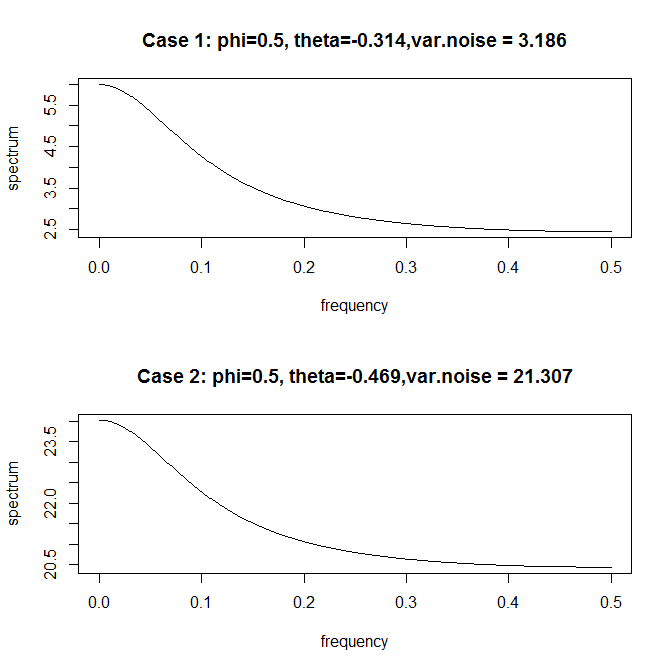
\includegraphics[width=10cm]{Figures/Problem5_1}
	\caption{Theoretical spectral density of the two ARMA(1,1) models}
	\label{fig:SpectralDensity2ARMA}
\end{figure}

\subsection{Simulating and Estimating the Spectra of two cases}
The simulation of 200 observations of the two ARMA(1,1) models is given in Figure \ref{fig:Simulation}. Their estimated spectra is given in Figure \ref{fig:EstimateSpectra}. I used the averaged periodogram as the smoothing method, with $L = 9$.

\begin{figure}
	\centering
	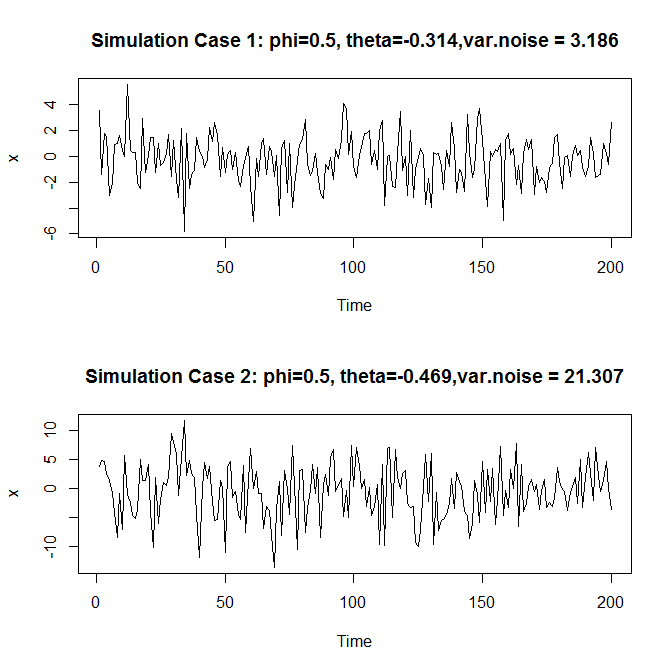
\includegraphics[width=9cm]{Figures/Problem5_2}
	\caption{Simulation of 200 observations of the two ARMA(1,1) models}
	\label{fig:Simulation}
\end{figure}

\begin{figure}
	\centering
	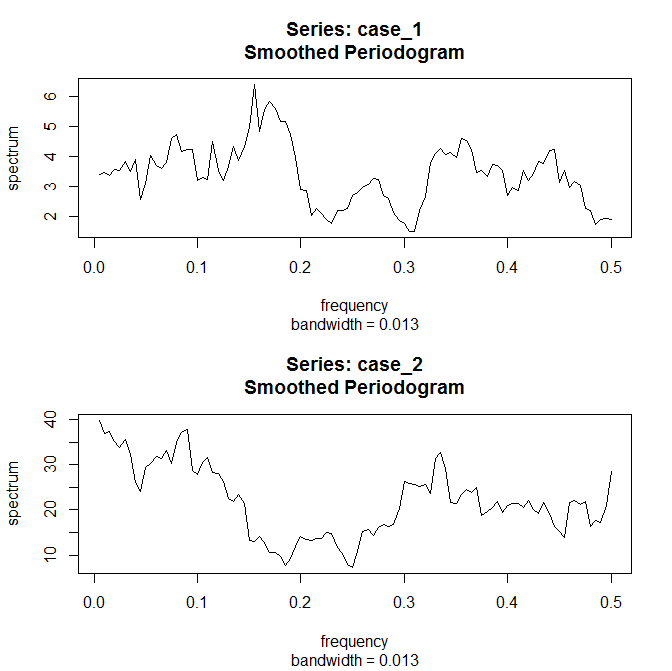
\includegraphics[width=9cm]{Figures/Problem5_3}
	\caption{Estimated spectra of the two ARMA(1,1) models, using averaged periodograms with $L=9$}
	\label{fig:EstimateSpectra}
\end{figure}

\end{document}